\section{Create a JavaScript Object}
Now, in order to display the content of the file, we decide to create an object, called $``metaSpecObject''$. This object is a generic object that can contains all the data to represent a molecule along with its spectrum and the information to allow the cross talk between the two entities.
    \begin{figure}[h]
    \begin{centering}
    \caption{Attributes of the metaSpecObject}

\includegraphics[width=195mm,height=150mm]{./images/metaSpecObjectAttributes}
%    \label{subd}
    \end{centering}
    \end{figure}
\clearpage

The aim is to conceive an object that holds all the elements to create a molecule object, a spectrum object, and keeping track of the relation between one peak and another object(either a molecule or an atom).
This is way, each peak is considered as being an object (@see peak.js) and has several fields that may relate to its corresponding objects:\\

    \begin{figure}[h]
    \begin{centering}
    \caption{The object Peak}
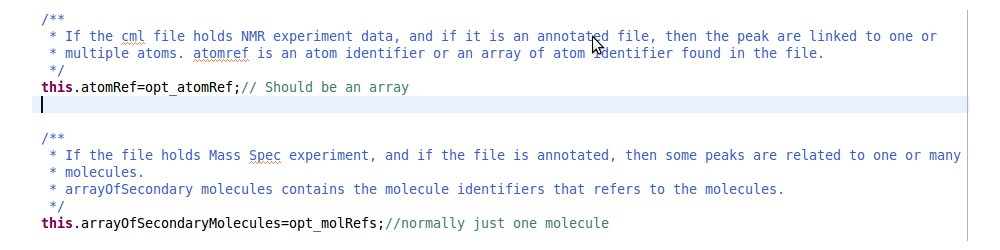
\includegraphics[width=195mm,height=50mm]{./images/peakAnnotation}
%    \label{subd}
    \end{centering}
    \end{figure}
With these two fields, whenever a peak is linked to another object,  it is possible to track this object.




\clearpage
